\documentclass{article}

  % packages
    % basic stuff for rendering math
    \usepackage[letterpaper, top=1in, bottom=1in, left=1in, right=1in]{geometry}
    \usepackage[utf8]{inputenc}
    \usepackage[english]{babel}
    \usepackage{amsmath} 
    \usepackage{amssymb}

    % extra math symbols and utilities
    \usepackage{mathtools}        % for extra stuff like \coloneqq
    \usepackage{mathrsfs}         % for extra stuff like \mathsrc{}
    \usepackage{centernot}        % for the centernot arrow 
    \usepackage{bm}               % for better boldsymbol/mathbf 
    \usepackage{enumitem}         % better control over enumerate, itemize
    \usepackage{hyperref}         % for hypertext linking
    \usepackage{fancyvrb}          % for better verbatim environments
    \usepackage{newverbs}         % for texttt{}
    \usepackage{xcolor}           % for colored text 
    \usepackage{listings}         % to include code
    \usepackage{lstautogobble}    % helper package for code
    \usepackage{parcolumns}       % for side by side columns for two column code
    

    % page layout
    \usepackage{fancyhdr}         % for headers and footers 
    \usepackage{lastpage}         % to include last page number in footer 
    \usepackage{parskip}          % for no indentation and space between paragraphs    
    \usepackage[T1]{fontenc}      % to include \textbackslash
    \usepackage{footnote}
    \usepackage{etoolbox}

    % for custom environments
    \usepackage{tcolorbox}        % for better colored boxes in custom environments
    \tcbuselibrary{breakable}     % to allow tcolorboxes to break across pages

    % figures
    \usepackage{pgfplots}
    \pgfplotsset{compat=1.18}
    \usepackage{float}            % for [H] figure placement
    \usepackage{tikz}
    \usepackage{tikz-cd}
    \usepackage{circuitikz}
    \usetikzlibrary{arrows}
    \usetikzlibrary{positioning}
    \usetikzlibrary{calc}
    \usepackage{graphicx}
    \usepackage{algorithmic}
    \usepackage{caption} 
    \usepackage{subcaption}
    \captionsetup{font=small}

    % for tabular stuff 
    \usepackage{dcolumn}

    \usepackage[nottoc]{tocbibind}
    \pdfsuppresswarningpagegroup=1
    \hfuzz=5.002pt                % ignore overfull hbox badness warnings below this limit

  % New and replaced operators
    \DeclareMathOperator{\Tr}{Tr}
    \DeclareMathOperator{\Sym}{Sym}
    \DeclareMathOperator{\Span}{span}
    \DeclareMathOperator{\std}{std}
    \DeclareMathOperator{\Cov}{Cov}
    \DeclareMathOperator{\Var}{Var}
    \DeclareMathOperator{\Corr}{Corr}
    \DeclareMathOperator{\pos}{pos}
    \DeclareMathOperator*{\argmin}{\arg\!\min}
    \DeclareMathOperator*{\argmax}{\arg\!\max}
    \newcommand{\ket}[1]{\ensuremath{\left|#1\right\rangle}}
    \newcommand{\bra}[1]{\ensuremath{\left\langle#1\right|}}
    \newcommand{\braket}[2]{\langle #1 | #2 \rangle}
    \newcommand{\qed}{\hfill$\blacksquare$}     % I like QED squares to be black

  % Custom Environments
    \newtcolorbox[auto counter, number within=section]{question}[1][]
    {
      colframe = orange!25,
      colback  = orange!10,
      coltitle = orange!20!black,  
      breakable, 
      title = \textbf{Question \thetcbcounter ~(#1)}
    }

    \newtcolorbox[auto counter, number within=section]{exercise}[1][]
    {
      colframe = teal!25,
      colback  = teal!10,
      coltitle = teal!20!black,  
      breakable, 
      title = \textbf{Exercise \thetcbcounter ~(#1)}
    }
    \newtcolorbox[auto counter, number within=section]{solution}[1][]
    {
      colframe = violet!25,
      colback  = violet!10,
      coltitle = violet!20!black,  
      breakable, 
      title = \textbf{Solution \thetcbcounter}
    }
    \newtcolorbox[auto counter, number within=section]{lemma}[1][]
    {
      colframe = red!25,
      colback  = red!10,
      coltitle = red!20!black,  
      breakable, 
      title = \textbf{Lemma \thetcbcounter ~(#1)}
    }
    \newtcolorbox[auto counter, number within=section]{theorem}[1][]
    {
      colframe = red!25,
      colback  = red!10,
      coltitle = red!20!black,  
      breakable, 
      title = \textbf{Theorem \thetcbcounter ~(#1)}
    } 
    \newtcolorbox[auto counter, number within=section]{proposition}[1][]
    {
      colframe = red!25,
      colback  = red!10,
      coltitle = red!20!black,  
      breakable, 
      title = \textbf{Proposition \thetcbcounter ~(#1)}
    } 
    \newtcolorbox[auto counter, number within=section]{corollary}[1][]
    {
      colframe = red!25,
      colback  = red!10,
      coltitle = red!20!black,  
      breakable, 
      title = \textbf{Corollary \thetcbcounter ~(#1)}
    } 
    \newtcolorbox[auto counter, number within=section]{proof}[1][]
    {
      colframe = orange!25,
      colback  = orange!10,
      coltitle = orange!20!black,  
      breakable, 
      title = \textbf{Proof. }
    } 
    \newtcolorbox[auto counter, number within=section]{definition}[1][]
    {
      colframe = yellow!25,
      colback  = yellow!10,
      coltitle = yellow!20!black,  
      breakable, 
      title = \textbf{Definition \thetcbcounter ~(#1)}
    } 
    \newtcolorbox[auto counter, number within=section]{example}[1][]
    {
      colframe = blue!25,
      colback  = blue!10,
      coltitle = blue!20!black,  
      breakable, 
      title = \textbf{Example \thetcbcounter ~(#1)}
    } 
    \newtcolorbox[auto counter, number within=section]{code}[1][]
    {
      colframe = green!25,
      colback  = green!10,
      coltitle = green!20!black,  
      breakable, 
      title = \textbf{Code \thetcbcounter ~(#1)}
    } 
    \newtcolorbox[auto counter, number within=section]{algo}[1][]
    {
      colframe = green!25,
      colback  = green!10,
      coltitle = green!20!black,  
      breakable, 
      title = \textbf{Algorithm \thetcbcounter ~(#1)}
    } 

    \BeforeBeginEnvironment{example}{\savenotes}
    \AfterEndEnvironment{example}{\spewnotes}
    \BeforeBeginEnvironment{lemma}{\savenotes}
    \AfterEndEnvironment{lemma}{\spewnotes}
    \BeforeBeginEnvironment{theorem}{\savenotes}
    \AfterEndEnvironment{theorem}{\spewnotes}
    \BeforeBeginEnvironment{corollary}{\savenotes}
    \AfterEndEnvironment{corollary}{\spewnotes}
    \BeforeBeginEnvironment{proposition}{\savenotes}
    \AfterEndEnvironment{proposition}{\spewnotes}
    \BeforeBeginEnvironment{definition}{\savenotes}
    \AfterEndEnvironment{definition}{\spewnotes}
    \BeforeBeginEnvironment{exercise}{\savenotes}
    \AfterEndEnvironment{exercise}{\spewnotes}
    \BeforeBeginEnvironment{proof}{\savenotes}
    \AfterEndEnvironment{proof}{\spewnotes}
    \BeforeBeginEnvironment{solution}{\savenotes}
    \AfterEndEnvironment{solution}{\spewnotes}
    \BeforeBeginEnvironment{question}{\savenotes}
    \AfterEndEnvironment{question}{\spewnotes}
    \BeforeBeginEnvironment{code}{\savenotes}
    \AfterEndEnvironment{code}{\spewnotes}
    \BeforeBeginEnvironment{algo}{\savenotes}
    \AfterEndEnvironment{algo}{\spewnotes}

    \definecolor{dkgreen}{rgb}{0,0.6,0}
    \definecolor{gray}{rgb}{0.5,0.5,0.5}
    \definecolor{mauve}{rgb}{0.58,0,0.82}
    \definecolor{darkblue}{rgb}{0,0,139}
    \definecolor{lightgray}{gray}{0.93}
    \renewcommand{\algorithmiccomment}[1]{\hfill$\triangleright$\textcolor{blue}{#1}}

    % default options for listings (for code)
    \lstset{
      autogobble,
      frame=ltbr,
      language=Python,
      aboveskip=3mm,
      belowskip=3mm,
      showstringspaces=false,
      columns=fullflexible,
      keepspaces=true,
      basicstyle={\small\ttfamily},
      numbers=left,
      firstnumber=1,                        % start line number at 1
      numberstyle=\tiny\color{gray},
      keywordstyle=\color{blue},
      commentstyle=\color{dkgreen},
      stringstyle=\color{mauve},
      backgroundcolor=\color{lightgray}, 
      breaklines=true,                      % break lines
      breakatwhitespace=true,
      tabsize=3, 
      xleftmargin=2em, 
      framexleftmargin=1.5em, 
      stepnumber=1
    }

  % Page style
    \pagestyle{fancy}
    \fancyhead[L]{Bayesian Inference}
    \fancyhead[C]{Muchang Bahng}
    \fancyhead[R]{Spring 2025} 
    \fancyfoot[C]{\thepage / \pageref{LastPage}}
    \renewcommand{\footrulewidth}{0.4pt}          % the footer line should be 0.4pt wide
    \renewcommand{\thispagestyle}[1]{}  % needed to include headers in title page

\begin{document}

\title{Bayesian Inference}
\author{Muchang Bahng}
\date{Spring 2025}

\maketitle
\tableofcontents
\pagebreak

This covers computability theory, complexity theory, and automata theory. 
Alphabet. Boolean logic

 
\section{Single Parameter Families} 

\subsection{Exponential Family}

\subsection{Conjugate Priors}

\subsection{Computing Posteriors with Beta Prior and Binomial Likelihood}

  The motivation behind the Beta distribution is that it satisfies \textbf{conjugacy} with a binomial likelihood. That is, assume that we have some data $\mathbf{x}$ of $N$ observations containing $m$ successes and $N-m$ failures (note that this observation $\mathbf{x}$ was in a way "reduced" to the information of only the number of successes $m$). We assume that there is some true success rate $\theta$ (between $0$ and $1$, of course) coming from these samples, and our job is to try and guess the true rate to the best of our abilities.

  Before we even observe the data $\mathbf{x}$, our initial guess of $\theta$ might be modeled by the prior distribution $\theta \sim \text{Beta}(a, b)$. Furthermore, the likelihood is clearly a binomial (since it represents the probability of getting $m$ successes out of $N$ samples with fixed rate of success $\theta$), so $m\,|\,\theta \sim \text{Binomial}(N, \theta)$. With these conditions, we claim that the posterior is also a beta, since
  \begin{align*}
    p(\theta\,|\, m) & \propto p_\theta (\theta) \, p(m\,|\,\theta) \\
    & \propto \theta^{a - 1} (1 - \theta)^{b - 1} \cdot \theta^m (1 - \theta)^{N - m} \\
    & = \theta^{a + m - 1} (1 - \theta)^{b + N - m - 1}
  \end{align*}

\subsection{Bayesian Inference for Gaussian}

  The maximum likelihood framework gave point estimates for the parameters $\mu$ and $\Sigma$. Now we develop a Bayesian treatment by introducing prior distributions over these parameters. Given a set of $N$ $D$-dimensional observations $\mathbf{X} = \{x_1, \ldots, x_n\}$, the likelihood function is given by (the unnormalized function of $\mu$):
  \begin{equation}
    p(\mathbf{X}\,|\,\mu, \Sigma) = \prod_{n=1}^N p(x_n\,|\,\mu, \Sigma) = \frac{1}{(2\pi)^{D/2}} \frac{1}{|\Sigma|^{1/2}} \exp \sum_{n=1}^N \bigg(-\frac{1}{2} (x_n - \mu)^T \Sigma^{-1} (x_n - \mu)\bigg)
  \end{equation}

  The likelihood function takes the form of the exponential of a quadratic form in $\mu$. Thus, if we choose a prior $p(\mu)$ given by a Gaussian, it will be a conjugate distribution for this likelihood function. Taking our prior distribution to be
  \begin{equation}
    p(\mu, \Sigma) = \mathcal{N}(\mu, \Sigma\,|\,\mu_0, \Sigma_0)
  \end{equation}

  The similarity of the symbols $\mu, \Sigma$ with $\mu_0, \Sigma_0$ may be slightly confusing. We can think as such: $\mu, \Sigma$ are random variables that determine the parameters of some Gaussian distribution. But the values $\mu, \Sigma$ are uncertain, and their possible values with probabilities take the form of another distribution $\mathcal{N}(\mu_0, \Sigma_0)$. The posterior distribution is given by the familiar formula
  \begin{equation}
    p(\mu, \Sigma\,|\,\mathbf{X}) \propto p(\mathbf{X}\,|\,\mu, \Sigma) \; p(\mu, \Sigma)
  \end{equation}

  which is another Gaussian $p(\mu\,|\,\mathbf{X}) = \mathcal{N}(\mu, \Sigma\,|\, \mu_N, \Sigma_N)$. Let us place a few conditions for simplification. Since every Gaussian density can be represented as a product of independent univariate Gaussians, we can work with univariate Gaussians. Furthermore, let us assume that the true value of $\sigma$ is known, so all we have to do is find the posterior distribution of $\mu$ using the prior density $\mathcal{N}(\mu\,|\,\mu_0, \sigma_0^2)$. We have our prior and likelihood to be the following. Note that while the likelihood distribution is pretty much given, we have the flexibility to choose what our prior distribution is. We have only set the prior as a Gaussian simply because it is a conjugate form and therefore will greatly simplify calculations.

  \begin{align*}
    p(\mu) & = \mathcal{N}(\mu\,|\,\mu_0, \sigma_0^2) = \frac{1}{\sqrt{2 \pi \sigma^2}} \exp\bigg(-\frac{1}{2\sigma^2} (\mu - \mu_0)^2) \bigg) \\
    p(\mathbf{X}\,|\,\mu) & = \prod_{n=1}^N p(x_n\,|\,\mu) = \frac{1}{(2 \pi \sigma^2)^{N/2}} \exp\bigg(-\frac{1}{2 \sigma^2} \sum_{n=1}^N (x_n - \mu)^2 \bigg)
  \end{align*}

  which gives a posterior $p(\mu\,|\,\mathbf{X}) = \mathcal{N}(\mu \,|\, \mu_N, \sigma_N^2)$ where
  \begin{align*}
    \mu_N & = \frac{\sigma^2}{N \sigma_0^2 + \sigma^2} \mu_0 + \frac{N \sigma_0^2}{N \sigma_0^2 + \sigma^2} \mu_{ML} \\
    \frac{1}{\sigma_N^2} & = \frac{1}{\sigma_0^2} + \frac{N}{\sigma^2}
  \end{align*}

  and $\mu_{ML}$ is the maximum likelihood solution for $\mu$ given by the sample mean $\mu_{ML} = \frac{1}{N} \sum_{n=1}^N x_n$. These values make sense. We can see that the mean of the posterior distribution $\mu_N$ is a compromise between the prior mean $\mu_0$ and maximum likelihood solution $\mu_{ML}$. If the number of observed data points $N=0$, then it is simply the prior mean, but for $N \rightarrow \infty$, the posterior mean is given by the maximum likelihood solution since the data ``overpowers'' the prior mean assumption.

  Now, suppose that the mean of the Gaussian over the data is known and we wish to infer the variance. For convenience, let us work with the precision $\lambda = \frac{1}{\sigma^2}$ over the variance. The likelihood function for $\lambda$ is
  \begin{equation}
    p(\mathbf{X}\,|\,\lambda) = \prod_{n=1}^N \mathcal{N} (x_n\,|\, \mu, \lambda^{-1}) \propto \lambda^{N/2} \exp \bigg(-\frac{\lambda}{2} \sum_{n=1}^N (x_n - \mu)^2 \bigg)
  \end{equation}

  Note that since this is a function of $\lambda$, it behaves differently than the likelihood function of $\mu$, even though they are of the same form. Since the likelihood function is proportional to the product of a power of $\lambda$ and the exponential of a linear function of $\lambda$, we must find a prior distribution $p(\lambda)$ with precisely these proportional properties identical to that of the likelihood. Fortunately, the Gamma distribution satisfies them, defined by
  \begin{equation}
    p(\lambda\,|\,a_0, b_0) = \text{Gamma}(\lambda\,|\, a_0, b_0) = \frac{1}{\Gamma(a_0)} b_0^{a_0} \lambda^{a_0-1} \exp(-b_0 \lambda)
  \end{equation}

  Using Bayes rule and multiplying gives the posterior density
  \begin{equation}
    p(\lambda\,|\,\mathbf{X}) \propto \lambda^{a_0 - 1} \lambda^{N/2} \exp\bigg( -b_0 \lambda - \frac{\lambda}{2} \sum_{n=1}^N (x_n - \mu)^2 \bigg)
  \end{equation}

  which is indeed the density of a $\text{Gamma}(\lambda\,|\,a_N, b_N)$ distribution, where
  \begin{align*}
    a_N & = a_0 + \frac{N}{2} \\
    b_N & = b_0 + \frac{1}{2} \sum_{n=1}^N (x_n - \mu)^2 = b_0 + \frac{N}{2} \sigma_{ML}^2
  \end{align*}

  where $\sigma_{ML}^2$ is the maximum likelihood estimator of the variance. Now, suppose that both the mean and precision are unknown. To find a conjugate prior, we consider the dependence of the likelihood function on $\mu$ and $\lambda$.
  \begin{align*}
    p(\mathbf{X}\,|\,\mu, \lambda) & = \prod_{n=1}^N \bigg(\frac{\lambda}{2\pi}\bigg)^{1/2} \exp \bigg( -\frac{\lambda}{2} (x_n - \mu)^2 \bigg) \\
    & \propto \bigg(\lambda^{1/2} \exp \Big(-\frac{\lambda \mu^2}{2} \Big) \bigg)^N \, \exp \bigg( \lambda \mu \sum_{n=1}^N x_n - \frac{\lambda}{2} \sum_{n=1}^N x_n^2 \bigg)
  \end{align*}

  We now wish to identify a prior distribution $p(\mu, \lambda)$ that has the same functional dependence on $\mu$ and $\lambda$ as the likelihood function and that should therefore take the form
  \begin{align*}
    p(\mu, \lambda) & \propto \bigg( \lambda^{1/2} \exp \Big(-\frac{\lambda \mu^2}{2}\Big) \bigg)^\beta \exp\big( c \lambda \mu - d \lambda \big) \\
    & = \exp \bigg( -\frac{\beta \lambda}{2} \Big(\mu - \frac{c}{\beta} \Big)^2 \bigg) \, \lambda^{\beta/2} \exp \bigg(-\Big(d - \frac{c^2}{2\beta}\Big) \lambda \bigg)
  \end{align*}

  where $c, d, \beta$ are constants. Since we can always write $p(\mu, \lambda) = p(\mu\,|\,\lambda) p(\lambda)$, we can find $p(\mu\,|\,\lambda)$ and $p(\lambda)$ by inspection. We have just shown that $p(\mu \,|\, \lambda)$ is a Gaussian whose precision is a linear function of $\lambda$ and that $p(\lambda)$ is a gamma distribution, so the normalized prior takes the form
  \begin{equation}
    p(\mu, \lambda) = \mathcal{N}(\mu \,|\, \mu_0, (\beta\lambda)^{-1}) \; \text{Gamma}(\lambda\,|\,a, b)
  \end{equation}

  which is called the \textbf{Gaussian-Gamma distribution}. Note that this is not simply the product of an independent Gaussian prior over $\mu$ and a gamma prior over $\lambda$, because the precision of $\mu$ is a linear function of $\lambda$. The extension of this to multivariate random variables is straightforward.

\subsection{Inference over Periodic Distributions}

  Although Gaussian distributions are of great significance, there are situations in which they are inappropriate as density models for continuous variables (e.g. wind direction or quantities periodic over 24 hours). Such quantities are conveniently represented using an angular (polar) coordinate $0 \leq \theta < 2\pi$. Let us consider the problem of evaluating the mean of a set of observations $\mathbf{\theta} = \{\theta_1, \theta_2, \ldots, \theta_N\}$ of a periodic variable measured in radians. The simple average $(\theta_1 + \ldots + \theta_N)/N$ is strongly coordinate dependent. To find an invariant measure of the mean, we can see that the observations can be viewed as points on the unit circle and can therefore be described instead by two-dimensional unit vectors $x_1, \ldots, x_N$, where $x_n = (\cos{\theta_n}, \sin{\theta_n})$. We can average these vectors and compute its angle to find this average angle.

  \begin{equation}
    \overline{x} = \frac{1}{N} \sum_{n=1}^N x_n = \Big( \frac{1}{N} \sum_{n=1}^N \cos{\theta_n} , \frac{1}{N} \sum_{n=1}^N \sin{\theta_n} \Big) \implies \overline{\theta} = \tan^{-1} \bigg( \frac{\sum_{n=1}^N \sin{\theta_n}}{\sum_{n=1}^N \cos{\theta_n}} \bigg)
  \end{equation}

  In general, any distribution $p(\theta)$ that have period $2\pi$ must be defined such that it is nonnegative, integrate to $1$, and be periodic.
  \begin{align*} 
    p(\theta) & \geq 0 \\
    \int_0^{2\pi} p(\theta)\,d\theta  & = 1 \\
    p(\theta + 2\pi) & = p(\theta)
  \end{align*}

  We can obtain a Gaussian-like distribution that satisfies these three properties. Consider a 2-dimensional Gaussian over variables $x_1, x_2$ having mean $\mu = (\mu_1, \mu_2)$ and a covariance matrix $\Sigma = \sigma^2 I$. This gives us
  \begin{equation}
    p(x_1, x_2) = \frac{1}{2\pi \sigma^2} \exp \bigg( -\frac{(x_1 - \mu_1)^2 + (x_2 - \mu_2)^2}{2\sigma^2} \bigg)
  \end{equation}

  Now, suppose that we consider the value of this distribution along a circle of fixed radius. Then, this distribution will be periodic, although it will not be normalized. We can determine the form of this distribution by transforming from Cartesian coordinates to polar coordinates $(r, \theta)$ (so that $x_1 = r \cos{\theta}, x_2 = r \sin{\theta}$) and keeping $r$ constant.

  \begin{figure}[H]
    \centering
    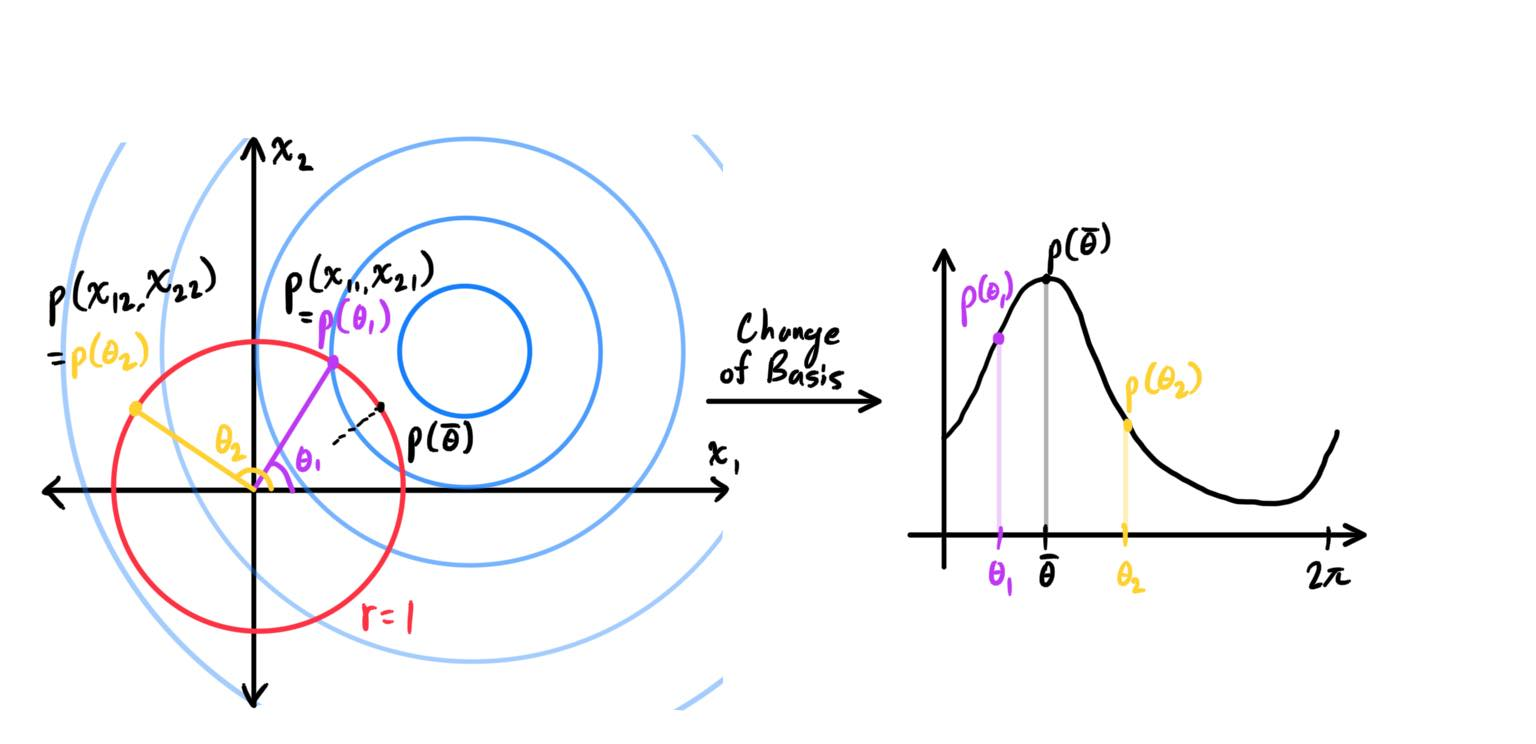
\includegraphics[width=0.7\textwidth]{img/circular_normal_change_of_basis.jpg}
    \caption{Circular normal change of basis}
  \end{figure}

  This transformation from $\mathbb{R}^2 \longrightarrow [0, 2\pi)$ defined
  \begin{equation}
    (x_1, x_2) \mapsto \tan^{-1} \frac{y}{x}
  \end{equation}
  simply takes the "circular" cross section of the Gaussian and maps those values.

  \begin{figure}[H]
    \centering
    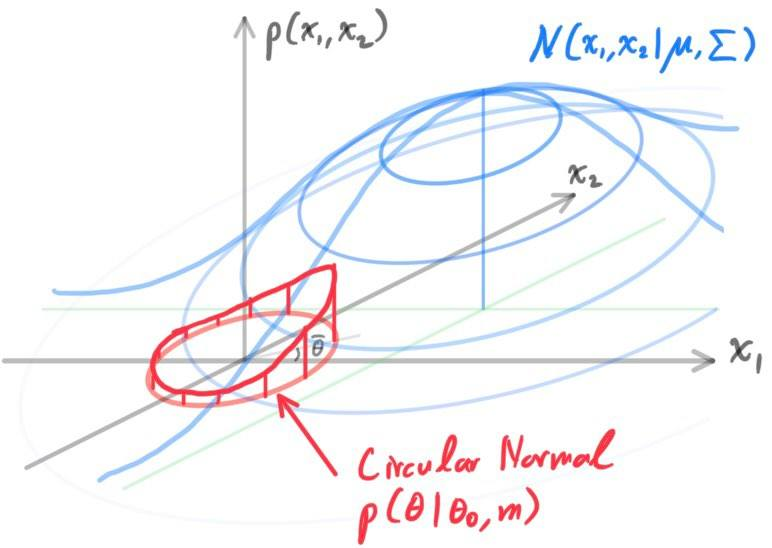
\includegraphics[width=0.5\textwidth]{img/Circular_Cross_Section.jpg}
    \caption{Circular cross section visualization}
  \end{figure}

  The value of $r$ is not important so we assume $r=1$. With some algebra and trig identities, we have the \textbf{circular normal}, or \textbf{von Mises distribution}, of form
  \begin{equation}
    p(\theta\,|\,\theta_0, m) = \frac{1}{2\pi I_0(m)} \exp \big( m \cos(\theta - \theta_0) \big)
  \end{equation}

  where the parameter $\theta_0$ corresponds to the mean of the distribution while $m$ is analogous to the precision for the Gaussian. The normalization coefficient $I_0(m)$ is the zeroth-order Bessel function of the first kind, defined by
  \begin{equation}
    I_0(m) = \frac{1}{2\pi} \int_0^{2\pi} \exp \big( m \cos{\theta}\big) \, d\theta
  \end{equation}

  For large $m$, the distribution becomes approximately Gaussian. Considering the maximum likelihood estimators for the parameters $\theta_0$ and $m$ for the circular normal, the log likelihood function is given by
  \begin{equation}
    \ln p(\mathbf{\theta}\,|\, \theta_0, m) = -N \ln(2\pi) - N \ln \big( I_0(m)\big) + m \sum_{n=1}^N \cos(\theta_n - \theta_0)
  \end{equation}

  The maximum estimator for the mean is
  \begin{equation}
    \theta_{0}^{ML} = \tan^{-1} \bigg( \frac{\sum_n \sin{\theta_n}}{\sum_n \cos{\theta_n}} \bigg)
  \end{equation}

  while that of $m$ can be evaluated numerically.

\subsection{Exponential Family of Distributions}

  The probability distributions so far are contained within the \textbf{exponential family} of distributions, which have important properties in common. The exponential family of distributions over $x \in \Omega \subset \mathbb{R}^D$, given parameters $\eta$, is defined to be the set of distributions of the form
  \begin{equation}
    p(x\,|\,\eta) = h(x) g(\eta) \exp\big(\eta^T u(x)\big)
  \end{equation}

  where $x$ may be a scalar or vector, discrete or continuous. Here, $\eta$ are called the \textbf{natural parameters} of the distribution, and $u(x)$ is some function of $x$. The function $g(\eta)$ can be interpreted as the normalizing coefficient and therefore satisfies
  \begin{equation}
    g(\eta) \int_{x \in \Omega} h(x) \exp\big(\eta^T u(x)\big) \, dx = 1
  \end{equation}

  with the integration replaced by a summation if $x$ is discrete.

  Now, consider a set of iid data denoted by $\mathbf{X} = \{x_1, \ldots, x_n\}$, for which the likelihood function is given by
  \begin{equation}
    p(X\,|\,\eta) = \bigg( \prod_{n=1}^N h(x_n) \bigg) g(\eta)^N\, \exp \bigg( \eta^T \sum_{n=1}^N u(x_n) \bigg)
  \end{equation}

  Setting the gradient of $\ln p(\mathbf{X}\,|\, \eta)$ with respect to $\eta$ to $0$, we can the following condition to be satisfied by the maximum likelihood estimator $\eta_{ML}$:
  \begin{equation}
    -\nabla \ln g(\eta_{ML}) = \frac{1}{N} \sum_{n=1}^N u(x_n)
  \end{equation}

  which can in principle be solved to obtain $\eta_{ML}$. The solution for the maximum likelihood estimator depends on the data only through $\sum_n u(x_n)$, which is therefore called the sufficient statistic of this distribution. Therefore, we do not need to store the entire data set itself but its sufficient statistic.

  In general, for a given probability distribution $p(\mathbf{X}\,|\, \eta)$, we can seek a prior that is conjugate to the likelihood function, so that the posterior distribution has the same functional form as the prior. Given that the likelihood function is in the exponential family, there exists a conjugate prior that can be written in the form
  \begin{equation}
    p(\eta) = p(\eta\,|\, \chi, \nu) = f(\chi, \nu) g(\eta)^\nu \exp \big( \nu \eta^T \chi \big)
  \end{equation}

  where $f(\chi, \nu)$ is a normalization coefficient, and $g(\eta)$ is the same function as the one appearing in the exponential family form of likelihood function. Indeed, multiplying this conjugate with the exponential family likelihood gives
  \begin{equation}
    p(\eta\,|\, \mathbf{X}, \chi, \nu) \propto g(\eta)^{\nu + N} \exp \Bigg( \eta^T \bigg( \sum_{n=1}^N u(x_n) + \nu \chi \bigg) \Bigg)
  \end{equation}


 
\include{sec/multi_parameter} 
\section{Bias Variance Decomposition}  

  The likelihood defines a proper loss function. Now let's try to parse the loss a bit more. It turns out that for a lot of popular loss functions, they generally decomposes into 
  \begin{equation}
    \text{Loss} = \text{Bias} + \text{Variance} + \text{Noise}
  \end{equation} 

  This decomposition is by no means exact, but it \textit{generally} holds true. This is formalized by deriving an exact decomposition of the MSE loss. This is possible because the MSE loss allows us to get an $L^2$ space, which allows for orthogonal decompositions. Unfortunately, when you have other losses, this becomes much messier because the inner product structure is not there. 

  In a more general case, when you take a supremum of risk over a function class, it decomposes into 3 terms. 
  \begin{enumerate}
    \item One of which quantifies how big the function class is (more variance). 
    \item One of which quantifies the distance between the truth and the function class (bias).  
    \item One is the noise term, which is the irreducible error. 
  \end{enumerate}

  \begin{example}[Bias and Variance Tradeoff in Polynomial Regression]
    Let's motivate this by trying to fit a polynomial on some data. 
    \begin{figure}[H]
      \centering 
      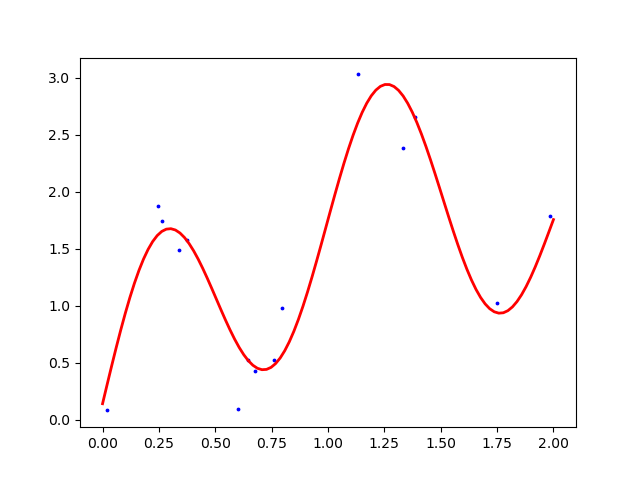
\includegraphics[scale=0.4]{img/True_data.png}
      \caption{A sample of $|\mathcal{D}| = 15$ data points are generated from the function $f(x) = \sin(2\pi x) + 2\cos (x - 1.5)$ with Gaussian noise $N(0, 0.3)$ on the interval $[0, 1]$. } 
      \label{fig:true_data}
    \end{figure}

    If we try to fit a polynomial function, how do we know which degree is best? Well the most simple thing is to just try all of them. To demonstrate this even further, I generated 10 different datasets  $\mathcal{D}$ of size $15$ taken from the same true distribution. The best fitted polynomials for each dataset is shown below. 

    \begin{figure}[H]
      \centering 
      \begin{subfigure}[b]{0.32\textwidth}
      \centering
        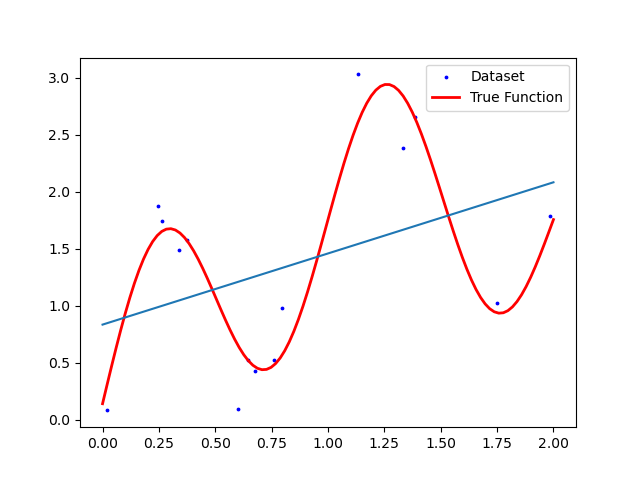
\includegraphics[width=\textwidth]{img/poly_1_fit.png}
        \caption{1st Degree}
        \label{fig:1d}
      \end{subfigure}
      \hfill 
      \begin{subfigure}[b]{0.32\textwidth}
      \centering
        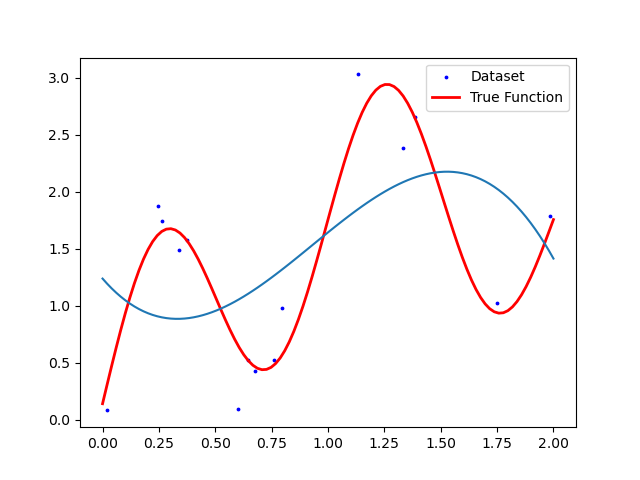
\includegraphics[width=\textwidth]{img/poly_3_fit.png}
        \caption{3rd Degree}
        \label{fig:3d}
      \end{subfigure}
      \hfill 
      \begin{subfigure}[b]{0.32\textwidth}
      \centering
        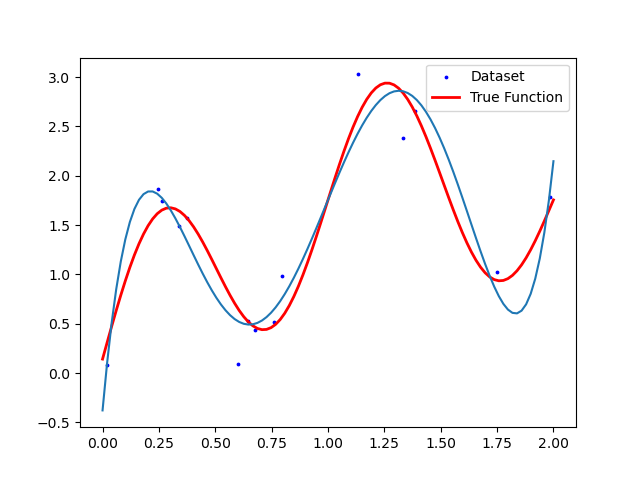
\includegraphics[width=\textwidth]{img/poly_5_fit.png}
        \caption{5th Degree}
        \label{fig:5e}
      \end{subfigure}

      \begin{subfigure}[b]{0.32\textwidth}
      \centering
        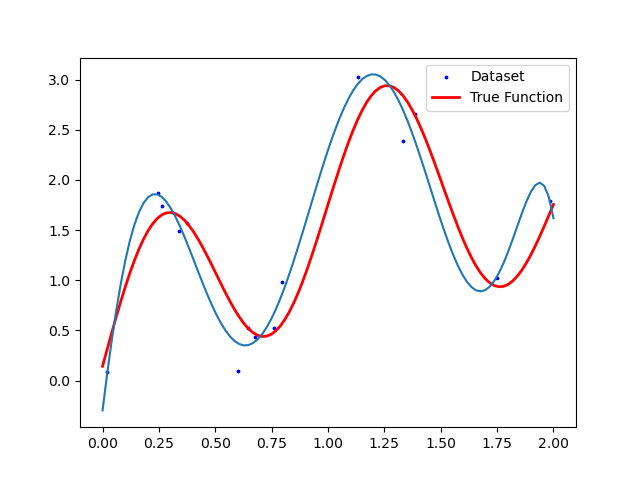
\includegraphics[width=\textwidth]{img/poly_7_fit.png}
        \caption{7th Degree}
        \label{fig:7d}
      \end{subfigure}
      \hfill 
      \begin{subfigure}[b]{0.32\textwidth}
      \centering
        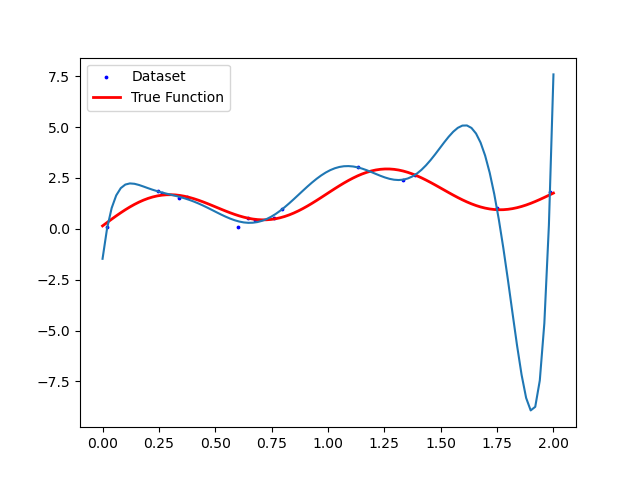
\includegraphics[width=\textwidth]{img/poly_9_fit.png}
        \caption{9th Degree}
        \label{fig:9d}
      \end{subfigure}
      \hfill 
      \begin{subfigure}[b]{0.32\textwidth}
      \centering
        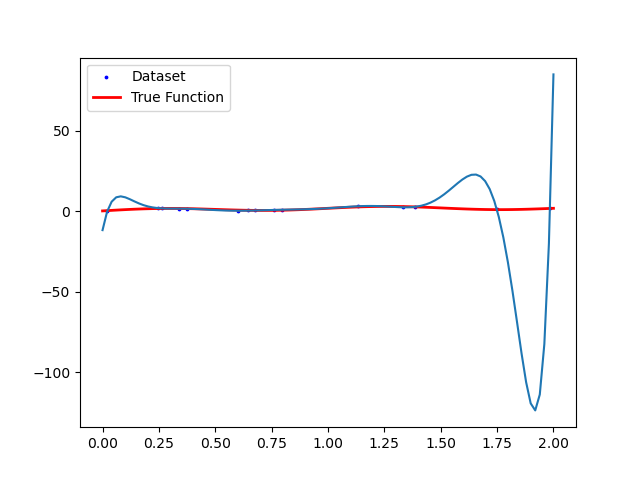
\includegraphics[width=\textwidth]{img/poly_11_fit.png}
        \caption{11th Degree}
        \label{fig:11e}
      \end{subfigure}

      \caption{Different model complexities (i.e. different polynomial degrees) lead to different fits of the data generated from the true distribution. The lower degree best fit polynomials don't have much variability in their best fits but have high bias, while the higher degree best fit polynomials have very high variability in their best fits but have low bias. The code used to generate this data is \href{code/polynomial_fitting.ipynb}{here}. }
      \label{fig:polynomial_fitting}
    \end{figure}

    We already know that the 5th degree approximation is most optimal, and the lower degree ones are \textbf{underfitting} the data, while the higher degree ones are \textbf{overfitting}. As mentioned before, we can describe the underfitting and overfitting phenomena through the bias variance decomposition. 

    \begin{enumerate}
      \item If we underfit the data, this means that our model is not robust and does not capture the patterns inherent in the data. It has a high bias since the set of function it encapsulates is not large enough to model $\mathbb{E}[Y\mid X]$. However, it has a low variance since if we were to take different samples of the dataset $\mathcal{D}$, the optimal parameters would not fluctuate. 

      \item What overfitting essentially means is that our model is too complex to the point where it starts to fit to the \textit{noise} of the data. This means that the variance is high, since different samples of the dataset $\mathcal{D}$ would cause huge fluctuations in the optimal trained parameters $\boldsymbol{\theta}$. However, the function set would be large, and thus it would be close to $\mathbb{E}[Y \mid X]$, leading to a low bias. 
    \end{enumerate}
  \end{example}
  
  \begin{example}[Polynomial Regression Continued]
    Another way to reduce the overfitting problem is if we have more training data to work with. That is, if we were to fit a 9th degree polynomial on a training set of not $N = 15$, but $N = 100$ data points, then we can see that this gives a much better fit. This makes sense because now the random variable $\mathcal{D}$, as a function of more random variables, has lower variance. Therefore, the lower variance in the dataset translates to lower variance in the optimal parameter. 

    \begin{figure}[H]
      \centering
      \begin{subfigure}[b]{0.48\textwidth}
      \centering
        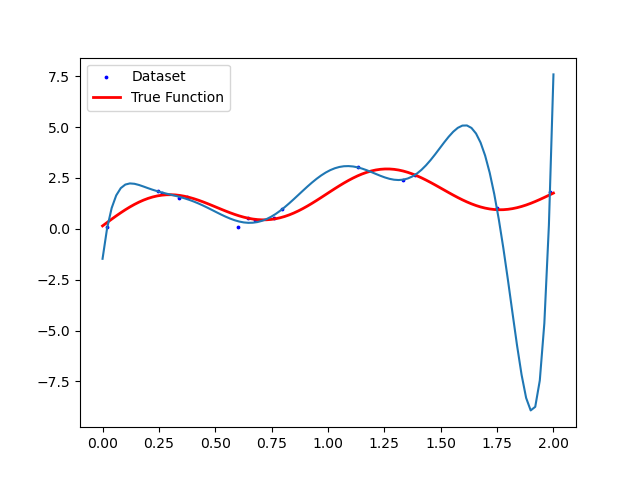
\includegraphics[width=\textwidth]{img/poly_9_fit.png}
        \caption{$M = 9, N = 15$}
        \label{fig:less_points}
      \end{subfigure}
      \hfill 
      \begin{subfigure}[b]{0.48\textwidth}
      \centering
        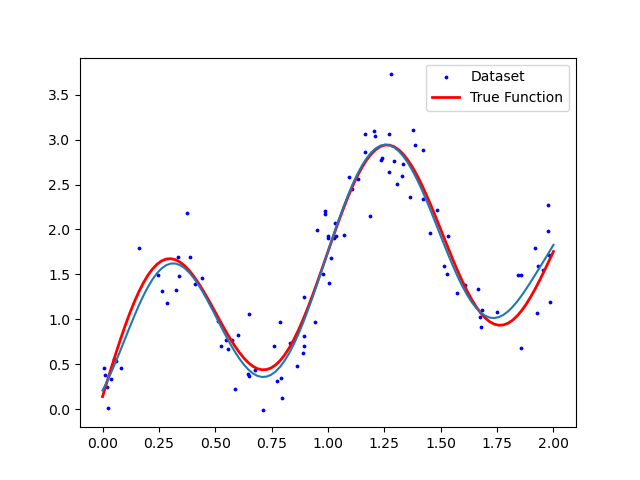
\includegraphics[width=\textwidth]{img/increased_data.png}
        \caption{$M = 9, N = 100$}
        \label{fig:more_points}
      \end{subfigure}
      \caption{Increasing the number of data points helps the overfitting problem. Now, we can afford to fit a 9th degree polynomial with reasonable accuracy.}
      \label{fig:reducing_overfitting_with_more_samples}
    \end{figure}
  \end{example}



\subsection{MSE Loss} 

  \begin{definition}[Mean Squared Error Loss]
    \label{mse_loss}
    The \textbf{MSE loss} is defined 
    \begin{equation}
      L(y, x) = (y - f(x))^2
    \end{equation}
  \end{definition}

  It is a well known fact that the true regressor---which may not be linear at all---that minimizes this loss is 
  \begin{equation}
    f^\ast (x) = \mathbb{E}[Y \mid X = x]
  \end{equation}
  which is the conditional expectation of $Y$ given $X$. This is the true regressor function, which is the best approximation of $Y$ over the $\sigma$-algebra generated by $X$. Therefore, if we consider a function class of linear predictors, we can decompose our risk, which is the distance between our estimated linear regressor and $Y$, as the sum of the distance between our estimator and the best regressor plus the distance between the best regressor and $Y$. 

  \begin{theorem}[Pythagorean's Theorem]
    The expected square loss over the joint measure $\mathbb{P}_{x, y}$ can be decomposed as 
    \begin{equation}
      \mathbb{E}_{x, y} [( y - f(x))^2] = \mathbb{E}_{x, y} [\big(y - \mathbb{E}[y \mid x]\big)^2] + \mathbb{E}_x [\big(\mathbb{E}[y \mid x] - h(x) \big)^2]
    \end{equation}
    That is, the squared loss decomposes into the squared loss of $\mathbb{E}[y \mid x]$ and $g(x)$, which is the intrinsic misspecification of the model, plus the squared difference of $y$ with its best approximation $\mathbb{E}[y \mid x]$, which is the intrinsic noise inherent in $y$ beyond the $\sigma$-algebra of $x$. 
  \end{theorem}
  \begin{proof}
    We can write 
    \begin{align}
      \mathbb{E}_{x, y} \big[ \big(y - f(x)\big)^2 \big] & = \mathbb{E}_{x, y}\big[ \big((y - \mathbb{E}[y \mid x]) + (\mathbb{E}[y \mid x] - f(x)) \big)^2 \big] \\
      & = \mathbb{E}_{x, y} [\big(y - \mathbb{E}[y \mid x]\big)^2] + \mathbb{E}_{x, y} [\{y - \mathbb{E} [y \mid x]\} \, \{ \mathbb{E}[y \mid x] - f(x) \}] \\
      & \;\;\;\;\;\;\;\;\;\;\;\;\;\;\; + \mathbb{E}_x [\big(\mathbb{E}[y \mid x] - f(x) \big)^2] \\
      & = \mathbb{E}_{x, y} [\big(y - \mathbb{E}[y \mid x]\big)^2] + \mathbb{E}_x [\big(\mathbb{E}[y \mid x] - f(x) \big)^2]
    \end{align}
    where the middle term cancels out due to the tower property. 
  \end{proof}

  Note that since $\mathbb{E}[\big(\mathbb{E}[Y \mid X] - g(X) \big)^2]$ is the misspecification of the model, we cannot change this (positive) constant, so $\mathbb{E}\big[ \big(Y - g(X)\big)^2 \big] \geq \mathbb{E}[(Y - \mathbb{E}[Y \mid X])^2]$, with equality achieved when we perfectly fit $g$ as $\mathbb{E}[Y \mid X]$ (i.e. the model is well-specified). Therefore, denoting $\mathcal{F}$ as the set of all $\sigma(X)$-measurable functions, then the minimum of the loss is attained when 
  \begin{equation}
    \argmin_{g \in \mathcal{F}} \mathbb{E}[L] = \argmin_{g \in \mathcal{F}} \mathbb{E} \big[ \big(Y - g(X)\big)^2 \big] = \mathbb{E}[Y \mid X]
  \end{equation}
  Essentially, we have decomposed our risk to a part that we can optimize and a part that we cannot, i.e. the intrinsic noise. 

  \begin{corollary}[Sufficient to Estimate Conditional Expectation]
    Minimizing the prediction risk is equivalent to minimizing the risk of our estimator to the conditional distribution. 
    \begin{equation}
      \argmin_{f \in \mathcal{F}} R(f) = \argmin_{f \in \mathcal{F}} \mathbb{E}_{x, y} \left[ (\mathbb{E}[y|x] - f(x))^2 \right]
    \end{equation}
  \end{corollary}
  
  Even though this example is specific for the mean squared loss, this same decomposition, along with the bias variance decomposition, exists for other losses. It just happens so that the derivations are simple for the MSE, which is why this is introduced first. However, the derivations for other losses are much more messy, and sometimes may not hold rigorously. However, the general intuition that more complex models tend to overfit (higher variance) still hold true. 

  Let's try to decompose this even more. In frequentist inference, we take a dataset $\mathcal{D}$ and optimize $\hat{f}$ that minimizes this empirical risk. Therefore, for a given $\mathcal{D}$, $\hat{f} = \hat{f}(\mathcal{D})$ is determined, and if $\mathcal{D} = (x^{(i)}, y^{(i)})^n$ is a random variable, then $\hat{f}$ is also a random variable, which we will denote as $\hat{f}_{\mathcal{D}}$ for clarity. It is useful to think of $\mathcal{D}$ as a random variable because by seeing how $\hat{f}_{\mathcal{D}}$ varies as the dataset changes, we can measure the uncertainty in our estimate of $\hat{f}_{\mathcal{D}}$ through $\mathcal{D}$.\footnote{If this didn't make sense to you, consider the following thought experiment. Suppose we had a large number of datasets each of size $N$ and each drawn independently from the joint distribution $X \times Y$. For any given dataset $\mathcal{D}$, we can run our learning algorithm and obtain our best fit function $\hat{f}_{\mathcal{D}}$. Different datasets from the ensemble will give different functions and consequently different values of the squared loss. }

  \begin{lemma}[Conditional Prediction Risk] 
    Our conditional prediction risk is 
    \begin{equation}
      r(\mathcal{D}) = \mathbb{E}_{x, y} \left[ (\mathbb{E}[y \mid x] - \hat{f}(x))^2 \mid \mathcal{D} \right]
    \end{equation}
    If $\mathcal{D}$ is fixed, then this is a real number. If $\mathcal{D}$ is a random variable, then this is a real-valued random variable. 
  \end{lemma} 

  Ideally, we would like two things. 
  \begin{enumerate}
    \item \textit{Low Bias}. The average prediction we get over all $\hat{f}_{\mathcal{D}}$ trained on all possible samples of dataset $\mathcal{D}$ should be similar to our best regressor. That is, 
    \begin{equation}
      \mathbb{E}_{\mathcal{D}} \left[ \mathbb{E}_{x, y} \left[ (\mathbb{E}[y \mid x] - \hat{f}_{\mathcal{D}}(x))^2 \right] \right]
    \end{equation}
    should be as low as possible. 

    \item \textit{Low Variance}. The variance of our conditional prediction risk  
    \begin{equation}
      \Var_{\mathcal{D}} \left[ \mathbb{E}_{x, y} \left[ (\mathbb{E}[y \mid x] - \hat{f}_{\mathcal{D}}(x))^2 \right] \right]
    \end{equation}
    should be as low as possible. That is, we may get very low bias for one dataset $\mathcal{D}$, but if we sampled a different dataset, we should not expect the bias to explode. 
  \end{enumerate}

  Unfortunately, having both low bias \textit{and} low variance is not possible, and we wish to show that now. 

  \begin{theorem}[Bias Variance Decomposition Under MSE Loss]
    The expected optimal MSE loss decomposes to 
    \begin{equation}
      \mathbb{E}_{\mathcal{D}} \left[ (\mathbb{E}[y \mid x] - \hat{f}_\mathcal{D} (x))^2 \right] = \underbrace{ \big( \mathbb{E}[y \mid x] - \mathbb{E}_{\mathcal{D}} [\hat{f}_\mathcal{D} (x)] \big)^2}_{(\text{bias of } \hat{f}_{\mathcal{D}})^2} + \underbrace{ \mathbb{E}_\mathcal{D} \big[ \big( \mathbb{E}_\mathcal{D} [\hat{f}_\mathcal{D} (x)] - \hat{f}_\mathcal{D} (x) \big)^2 \big]}_{\text{variance of } \hat{f}_{\mathcal{D}}}
    \end{equation}
  \end{theorem}
  \begin{proof}
    Consider the term $\big(\mathbb{E}[y \mid x] - \hat{f}_{\mathcal{D}}(x) \big)^2$ above, which models the discrepancy in our optimized hypothesis and the best approximation. We take $\mathbb{E}_{\mathcal{D}} [ \hat{f}_{\mathcal{D}} (x)]$\footnote{Over all datasets $\mathcal{D}$, there will be a function $h_{{\boldsymbol{\theta}}; \mathcal{D}}$, and averaged over all datasets $\mathcal{D}$ is $\mathbb{E}_\mathcal{D} [ \hat{f}_{\mathcal{D}}]$. } So we can split the term into 

    \begin{align}
      \big(\mathbb{E}[y \mid x] - \hat{f}_{\mathcal{D}} (x) \big)^2 & =  \big[ \big( \mathbb{E}[y \mid x] - \mathbb{E}_\mathcal{D} [\hat{f}_{\mathcal{D}} (x)] \big) + \big( \mathbb{E}_\mathcal{D} [\hat{f}_{\mathcal{D}} (x)] - \hat{f}_{\mathcal{D}} (x) \big) \big]^2 \\
      & = \big( \mathbb{E}[y \mid x] - \mathbb{E}_\mathcal{D} [\hat{f}_{\mathcal{D}} (x)] \big)^2 + \big( \mathbb{E}_\mathcal{D} [\hat{f}_{\mathcal{D}} (x)] - \hat{f}_{\mathcal{D}} (x) \big)^2 \\
      & \;\;\;\;\;\;\;\; + 2 \big( \mathbb{E}[y \mid x] - \mathbb{E}_\mathcal{D} [\hat{f}_{\mathcal{D}} (x)] \big) \big( \mathbb{E}_\mathcal{D} [\hat{f}_{\mathcal{D}} (x)] - \hat{f}_{\mathcal{D}} (x) \big) 
    \end{align}

    Now take the expectation over $\mathcal{D}$, and for the third term, note that $\big( \mathbb{E}[y \mid x] - \mathbb{E}_\mathcal{D} [\hat{f}_{\mathcal{D}} (x)] \big)$ is constant with respect to $\mathbb{D}$ anyways, so we can take it out of the expectation. Therefore, 
    \begin{align}
      \mathbb{E}_{\mathcal{D}} \big[ \big( \mathbb{E}[y \mid x] - & \mathbb{E}_\mathcal{D} [\hat{f}_{\mathcal{D}} (x)] \big) \big( \mathbb{E}_\mathcal{D} [\hat{f}_{\mathcal{D}} (x)] - \hat{f}_{\mathcal{D}} (x) \big) \big] \\
      & = \big( \mathbb{E}[y \mid x] - \mathbb{E}_\mathcal{D} [\hat{f}_{\mathcal{D}} (x)] \big) \, \mathbb{E}_{\mathcal{D}} \big[ \mathbb{E}_\mathcal{D} [\hat{f}_{\mathcal{D}} (x)] - \hat{f}_{\mathcal{D}} (x) \big] \\ 
      & = \big( \mathbb{E}[y \mid x] - \mathbb{E}_\mathcal{D} [\hat{f}_{\mathcal{D}} (x)] \big) \cdot 0 = 0
    \end{align} 
  \end{proof} 

  Let's parse these terms a bit more. 
  \begin{enumerate}
    \item The bias $\mathbb{E}[y \mid x] - \mathbb{E}_{\mathcal{D}} [\hat{f}_\mathcal{D} (x)]$ is a random variable of $x$ that measures the difference between the average of our learned predictor $\mathbb{E}_{\mathcal{D}} [\hat{f}_\mathcal{D} (x)]$ and the true regressor $\mathbb{E}[y \mid x]$. 

    \item The variance $\mathbb{E}_\mathcal{D} \big[ \big( \mathbb{E}_\mathcal{D} [\hat{f}_\mathcal{D} (x)] - \hat{f}_\mathcal{D} (x) \big)^2 \big]$ is a random variable of $x$ that measures the variability of our learned functions $\hat{f}_{\mathcal{D}}$ around our mean $\mathbb{E}_\mathcal{D} [\hat{f}_\mathcal{D} (x)]$. 
  \end{enumerate}

  Therefore, we can substitute this back into our Pythagoras decomposition, where we must now take the expected bias and the expected variance over $x$ to get a form like 
  \begin{equation}
    \text{Expected Loss} = (\text{Expected Bias})^2 + \text{Expected Variance} + \text{Noise}
  \end{equation}

  \begin{corollary}[Bias Variance Decomposition of Expected MSE Loss] 
    \label{bias_variance_mse}
    The expected optimal MSE loss decomposes to 
    \begin{align}
      \mathbb{E}_{\mathcal{D}} \mathbb{E}_{x, y} \big[ (y - \hat{f}_{\mathcal{D}}(x))^2 \big] 
      & = \mathbb{E}_{x} \big[ \underbrace{ \big( \mathbb{E}[y \mid x] - \mathbb{E}_{\mathcal{D}} [\hat{f}_\mathcal{D} (x)] \big)^2}_{\text{(expected bias)}^2} \big] + \underbrace{ \mathbb{E}_\mathcal{D} \big[ \mathbb{E}_{x} \big[ \big( \mathbb{E}_\mathcal{D} [\hat{f}_\mathcal{D} (x)] - \hat{f}_\mathcal{D} (x) \big)^2 \big] \big]}_{\text{expected variance}} \\ 
      & \;\;\;\;\;\;\;\;\;\;\;\;\;\;\;\;\;\;\;\;\;\;\;\;\; + \underbrace{\mathbb{E}_{x, y} [(y - \mathbb{E}[y \mid x])^2]}_{\text{noise}}
    \end{align}
  \end{corollary}
  \begin{proof}
    By taking the expectation over $x$ and swapping the expectations (since $x$ and $\mathcal{D}$ are independent), and finally substituting back to Pythagoras decomposition, we get the following. 
  \end{proof}
  
\subsection{MAE Loss} 

  


\section{Hierarchical Modeling}

  Given a training data set $\mathcal{D} = (\mathbf{X}, \mathbf{Y})$ comprised of $N$ pairs of observations with corresponding target variables $\{(x_i, y_i)\}_{i=1}^N$ ($x_i \in \mathbb{R}^D, y_i \in \mathbb{R}$), the goal is to predict the value of $y$ for a new value of $x$. We first construct a \textit{statistical model} (more explained in next next subsection) by assuming that there exists some function $f(x)$ of some form such that the $y_i$'s have been generated by inputting the $x_i$'s into $f$, followed by a random residual term. We assume that the data $\mathcal{D}$ has been sampled independently, but this may not always be a justifiable assumption in practice. Under this model, which we denote $\mathcal{M}_i$, we further assume that $f$ can be parameterized by a vector $\theta$, so therefore, we assume that
  \begin{equation}
    y = f(x, \theta) + \epsilon, \;\;\;\;\;\; \epsilon \sim \text{Residual} (\beta)
  \end{equation}
  where $\beta$ is some collection of parameters that determine the error function.

  \begin{itemize}
    \item The frequentist perspective reduces this problem to finding the value of $\theta$ that maximizes the likelihood. That is, we must find
    \begin{equation}
      \theta^* = \text{arg}\, \max_{\theta} p(\mathcal{D}\,|\,\theta) = \text{arg}\, \max_{\theta} \prod_{i=1}^N p(y_i \,|\,x_i, \theta)
    \end{equation}
    and claiming that $y = f(x, \theta^*)$ is the function of best fit. This is a quite straightforward (hopefully convex) optimization problem, which can be done in many ways (e.g. batch/sequential gradient descent, solving normal equations, etc.).

    \item The Bayesian approach attempts to construct a \textit{distribution} of the values of $\theta$. Clearly, this vector $\theta$ would be an element in some multidimensional Euclidean space, and we want to define a posterior density $p(\theta\,|\,\mathcal{D})$ across this space that tells us the probability of $\theta$. Using Bayes rule,
    \begin{equation}
      p(\theta\,|\,\mathcal{D}) \propto p(\mathcal{D}\,|\,\theta) \, p(\theta)
    \end{equation}
    we see that we must define some prior distribution $p(\theta)$ on $\theta$. We can assume that this prior is defined with some distribution
    \begin{equation}
      \theta \sim \text{Dist}_\theta (\gamma)
    \end{equation}
    where $\gamma$ is a collection of parameters on $\theta$. Knowing this prior of $\theta$ will allow us to get the posterior of $\theta\,|\,\mathcal{D}$. The not-so-complete Bayesian treatment would treat this $\gamma$ as a known constant. But note that there is still uncertainty of whether $\theta$ comes from $\text{Dist}_\theta (\gamma)$ for one value of $\gamma$, compared to another value of $\gamma$. This uncertainty requires us to treat $\gamma$ as now a \textbf{hyperparameter}, that is a parameter for the distribution of a parameter, and this distribution of $\gamma$, which we can denote
    \begin{equation}
      \gamma \sim \text{Dist}_\gamma (\xi)
    \end{equation}
    is called a \textbf{hyperprior}. We can construct higher and higher level hyperpriors on top of this as much as we want, which will lead to more flexibility in our model (but more computationally expensive). This is known as \textbf{hierarchical priors}. Generally, we will only go up to the level of one hyperparameter.
  \end{itemize}

  Let us summarize how we would conduct the Bayesian method step by step. We first have to determine how many levels of hierarchical priors we are accounting for. Say that we will treat $\xi$ as a constant, and consider the parameter $\theta$ along with its hyperparameter $\gamma$. Our goal is to compute the posterior $p(\theta\,|\,\mathcal{D})$.

  \begin{enumerate}
    \item Since there is uncertainty over the value of $\theta$ depending on $\gamma$, we can marginalize over $\gamma$ to get
    \begin{equation}
      p(\theta\,|\,\mathcal{D}) = \int p(\theta\,|\,\mathcal{D}, \gamma)\, p(\gamma\,|\,\mathcal{D})\; d\gamma
    \end{equation}
    If the situation calls for it, we could also compute the posterior by doing Bayes rule first to get $p(\theta\,|\,\mathcal{D}) \propto p(\mathcal{D}\,|\,\theta)\; p(\theta)$, but then we would have to calculate both $p(\mathcal{D}\,|\,\theta)$ and $p(\theta)$ by marginalizing each over $\gamma$, which would lead to complications.

    \item To calculate $p(\theta\,|\,\mathcal{D}, \gamma)$, note that the formula for the posterior density of $\theta$ given $\mathcal{D}$ is $p(\theta\,|\,\mathcal{D}) \propto p(\mathcal{D}\,|\,\theta) p(\theta)$, where $p(\theta)$ is a density function of $\theta$ and parameter $\gamma$, which means that $p(\theta\,|\,\mathcal{D})$ would be a density function of $\theta$ and parameter $\gamma$. But since $\gamma$ is fixed, the posterior
    \begin{equation}
      p(\theta\,|\,\mathcal{D}, \gamma) \propto p(\mathcal{D}\,|\,\theta, \gamma) p(\theta\,|\,\gamma)
    \end{equation}
    is a density function of $\theta$ with fixed constant $\gamma$. This can be easily calculated because the prior $p(\theta\,|\,\gamma)$ is of distribution $\text{Dist}_\theta (\gamma)$ and the likelihood $p(\mathcal{D}\,|\,\theta, \gamma)$ is the product of densities of $y$ given fixed $\theta$.

    \item To calculate $p(\gamma\,|\,\mathcal{D})$, we first use Bayes rule to get
    \begin{equation}
      p(\gamma\,|\,\mathcal{D}) \propto p(\mathcal{D}\,|\,\gamma)\, p(\gamma)
    \end{equation}
    This can be easily calculated because the prior $p(\gamma)$ is of distribution $\text{Dist}_\gamma (\xi)$ of given $\xi$. The likelihood can be marginalized over $\theta$ to get
    \begin{equation}
      p(\mathcal{D}\,|\,\gamma) = \int p(\mathcal{D}\,|\,\theta, \gamma)\, p(\theta\,|\, \gamma)\; d\theta
    \end{equation}
    where $p(\theta\,|\,\gamma)$ is a function of $\theta$ with given parameter $\gamma$, and $p(\mathcal{D}\,|\,\theta)$ is the product of the individual likelihoods.
  \end{enumerate}

  But remember that this was all assumed under model $\mathcal{M}_i$, so the posterior density $p(\theta^i \,|\,\mathcal{D})$ of the $\theta^i$ parameterizing our best-fit function is really
  \begin{equation}
    p(\theta^i \,|\,\mathcal{D}, \mathcal{M}_i)
  \end{equation}
  where we index the parameter of model $\mathcal{M}_i$ to be $\theta^i$, with a superscript (since we may mistake subscript indices to be the components of $\theta$).

 

\bibliography{./bibfile}
\bibliographystyle{alpha}
\end{document}
